\documentclass[UKenglish, dvipsnames]{beamer}
\usepackage[utf8]{inputenx} % For æ, ø, å
\usepackage{csquotes}       % Quotation marks
\usepackage{microtype}      % Improved typography
\usepackage{amssymb}        % Mathematical symbols
\usepackage{mathtools}      % Mathematical symbols
\usepackage[absolute, overlay]{textpos} % Arbitrary placement
\usepackage[export]{adjustbox}
\usepackage{tikz}
\usepackage{acro} % for acronyms
\usepackage{graphicx}
\usepackage{xcolor}
\usepackage{subcaption} % for inserting side-by-side figures inside a figure environment
\usepackage{caption} % for better caption
\usepackage{tabularx}

% Beamer theme
\usetheme{UiB}

\setlength{\TPHorizModule}{\paperwidth} % Textpos units
\setlength{\TPVertModule}{\paperheight} % Textpos units
\usetikzlibrary{overlay-beamer-styles}  % Overlay effects for TikZ
% set captions with numbers
\setbeamertemplate{caption}[numbered]

\graphicspath{
    {./frames/figures/}
        {./content/chapter_1/images/}
        {./content/chapter_2/images/}
        {./content/chapter_3/images/}
        {./content/chapter_4/images/}
}

\acsetup{
    % format / first-long =   \emph,
    format / replace    =   true,
    single              =   true,
    single-style        =   long
}

% How to center a specific caption
\captionsetup{justification=centering}

% Document details
\author[Damiano Gianotti]{Damiano Gianotti}
\title{Remote and Continuous\\ Data Analysis}
\subtitle{For critical assets}
\date{13 aprile 2022}

% acro package configuration and acronym definitions
\acsetup{
    % make-links          =   true,
    % link-only-first     =   true,  %If this is activated then every short or alternative appearance of an acronym will be linked to its description in the list of acronyms.
    % pages / display     =   first,
    % pages / fill        =   {, },
    % format / first-long =   \emph,
    % format / replace    =   true
    % single              =   true,
    % single-style        =   long
}

% Chapter 1
% Data Analysis
\DeclareAcronym{BI}{
    short   =   {BI},
    long    =   {Business Intelligence}
}
\DeclareAcronym{DM}{
    short   =   {DM},
    long    =   {Data mining}
}
\DeclareAcronym{CRISP}{
    short   =   {CRISP},
    long    =   {Cross-industry standard process}
}
\DeclareAcronym{EDA}{
    short   =   {EDA},
    long    =   {Exploratory data analysis}
}
\DeclareAcronym{CDA}{
    short   =   {CDA},
    long    =   {Confirmatory data analysis}
}
\DeclareAcronym{KPIs}{
    short   =   {KPIs},
    long    =   {Key Performance Indicators}
}

% Maintenance
\DeclareAcronym{cmms}{
    short   =   {CMMS},
    long    =   {Computerized Maintenance Management Systems}
}
\DeclareAcronym{PM}{
    short   =   {PM},
    long    =   {Preventive maintenance}
}
\DeclareAcronym{ppm}{
    short   =   {PPM},
    long    =   {Planned preventive maintenance}
}
\DeclareAcronym{PdM}{
    short   =   {PdM},
    long    =   {Predictive maintenance}
}
\DeclareAcronym{cbm}{
    short   =   {CBM},
    long    =   {Condition-based maintenance}
}
\DeclareAcronym{cm}{
    short   =   {CM},
    long    =   {Condition monitoring}
}
\DeclareAcronym{mro}{
    short   =   {MRO},
    long    =   {Maintenance, repair and overhaul}
}
\DeclareAcronym{AI}{
    short   =   {AI},
    long    =   {Artificial Intelligence}
}
\DeclareAcronym{IoT}{
    short   =   {IoT},
    long    =   {Internet Of Things}
}
\DeclareAcronym{ML}{
    short   =   {ML},
    long    =   {Machine Learning}
}
\DeclareAcronym{infra}{
    short   =   {$\text{Infralytics}^\copyright$},
    long    =   {Infrastructure Analytics}
}

% Chapter 2
\DeclareAcronym{SaaS}{
    short   =   {SaaS},
    long    =   {Service as a Service}
}
\DeclareAcronym{IPCs}{
    short   =   {IPCs},
    long    =   {Industrial Personal Computers}
}
\DeclareAcronym{AWS}{
    short   =   {AWS},
    long    =   {Amazon Web Services}
}
\DeclareAcronym{S3}{
    short   =   {S3},
    long    =   {Simple Storage Service}
}

% Chapter 3
\DeclareAcronym{crud}{
    short   =   {CRUD},
    long    =   {Create Read Update Delete}
}
\DeclareAcronym{tsdb}{
    short   =   {TSDB},
    long    =   {Time Series Database}
}

%% Examples
\DeclareAcronym{gps}{
    short   =   {GPS},
    long    =   {Global Positioning System}
}
\DeclareAcronym{api}{
    short   =   {API},
    long    =   {Application Programming Interface}
}


\begin{document}

\section{Overview}
\begin{frame}{Table of contents}
    % Use
    %
    %     \begin{frame}[allowframebreaks]
    %
    % if the TOC does not fit one frame.
    \tableofcontents[currentsection]
\end{frame}

\section{Introduction}
\SectionPage

% \subsection{Data analysis}
\begin{frame}
    \frametitle{Data analysis}
    \vspace*{\fill}

    \begin{columns}[onlytextwidth, c]
        % Column 1
        \begin{column}{0.495\textwidth}
            \begin{itemize}
                % \item Process of \structure{breaking down} a whole into its constituent parts for closer evaluation.
                \item Process of breaking down whole into its parts % for closer evaluation.
                % \item Goal: closer evaluation 
                \item Has several dimension, names and approaches 
                % \item A wide range of techniques available % various \structure{names} and applied in a variety of
                \item Applicable to business, science, and social science sector
                \item Scientific method's extension 
            \end{itemize}
        \end{column}
        % Column 2    
        \begin{column}{0.495\textwidth}
            \includegraphics<1->[width=\textwidth]{Data_visualization_process_v1.png}
            % \caption{Data science process flowchart}
        \end{column}
    \end{columns}
    \vspace*{\fill}
\end{frame}

% \subsection{Operational environment}
\begin{frame}
    \frametitle{Operational environment: Maintenance}
    \vspace*{\fill}
    %In the numerous areas in which data analysis shines, 
    We focus on \structure{Maintenance}, where the
    priority is ensuring system reliability and safety during life cycles.
    The basic types are: % of maintenance
    \pause
    \begin{enumerate}
        \item \textbf{Reinforcement} % where equipment is reinforced and hardened to prevent failure
        \item \textbf{Corrective maintenance} % where equipment is repaired or replaced after wear, malfunction or break down
        \item \textbf{Preventive maintenance} % where equipment is checked and serviced in a planned manner; three subtypes:
    \end{enumerate}

    \pause
    \structure{Preventive maintenance} can be further divided into 3 types:
    \pause
    \begin{enumerate}% preventive, predictive, and prescriptive 
        \item[(A)] \acl{ppm} %calendar or usage based
        \item[(B)] \acl{PdM} %based on historical data
        \item[(C)] \acl{cbm} %\textit{maintenance when it is needed}
    \end{enumerate}

    \vspace*{\fill}
\end{frame}


\section{Host: Zensor}
\SectionPage
\begin{frame}{Table of contents}
    \tableofcontents[currentsection]
\end{frame}

\begin{frame}
    \frametitle{Zensor}

    \begin{alertblock}{Quick Overview}
        Based in Brussels, \alert{Belgium}. Main focus is \acs{IoT} and Industry 4.0.
        %, also operating in The Netherlands \& Germany 
    \end{alertblock}

    Provide a full, integrated, and intelligent monitoring solutions for:
    \begin{itemize}
        \item Industrial Production (Food, Glass, Metal)
        \item Infrastructure (Rail, Tram, Bridges)
        \item Renewable Energy (Offshore wind)
    \end{itemize}

    \pause
    \medskip
    Four aspect are involved:
    \begin{figure}[ht]
        \centering
        \includegraphics<2>[width=\textwidth]{4_phases_building_blocks.png}
        \caption{Project building blocks}
    \end{figure}

    \begin{textblock}{1}(0.015, 0.84)
        
\includegraphics[width = 2cm]{frames/logos/zensor_logo.png}
    \end{textblock}
\end{frame}

\begin{frame}
    \frametitle{Core Service}
    \begin{figure}[ht]
        \centering
        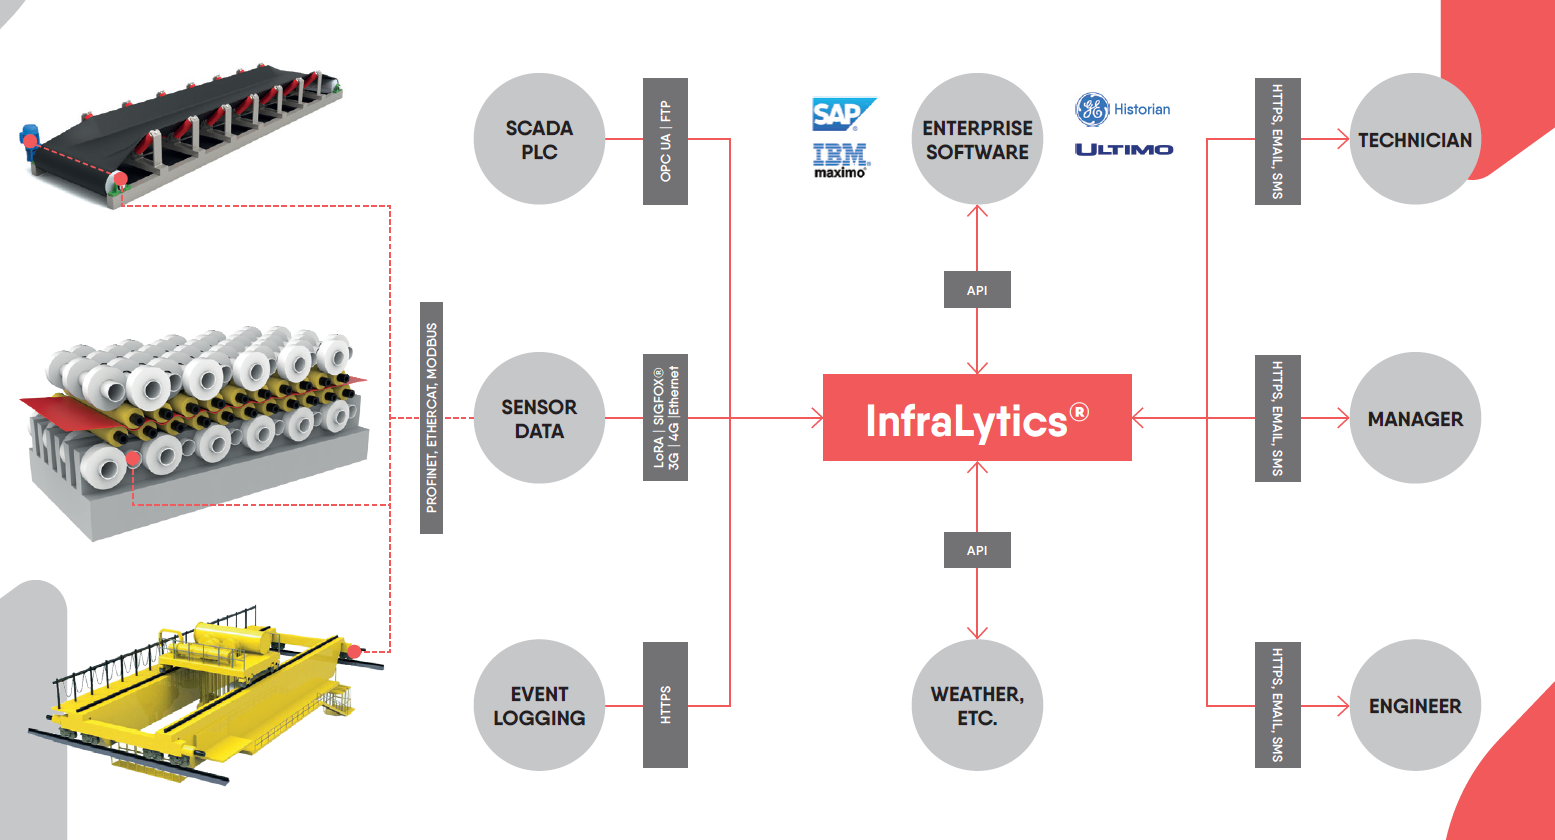
\includegraphics[width=0.98\textwidth]{how_it_works_plan_owner.png}
        \caption{\acl{infra} platform}
    \end{figure}

    \begin{textblock}{1}(0.015, 0.84)
        
\includegraphics[width = 2cm]{frames/logos/zensor_logo.png}
    \end{textblock}
\end{frame}
\section{Data analysis tools}
\SectionPage

\begin{frame}
    \frametitle{Data analysis tools}
    \vspace*{\fill}
    \begin{columns}[onlytextwidth, t]
        \begin{column}{.33\textwidth}
            \centering
            \textcolor{Aquamarine}{\Large Pandas}
            \vspace{0.5cm}

            \begin{itemize}
                \item Data processing \& cleaning
                \item Python library, widley adopted
                \item \textit{Split-Apply-Combine} approach
            \end{itemize}
        \end{column}

        \begin{column}{.33\textwidth}
            \centering
            \textcolor{YellowOrange}{\Large InfluxDB}
            \vspace{0.5cm}

            \begin{itemize}
                \item Data storage \& warehouse
                \item Key-value -- \acl{tsdb}
                \item TS-data that represent how a system changes (over time)
            \end{itemize}
        \end{column}

        % % vertical line
        % \begin{column}{.02\textwidth}
        %     \rule{.1mm}{0.7\textheight}
        % \end{column}

        \begin{column}{.33\textwidth}
            \centering
            \textcolor{violet}{\Large Grafana}
            \vspace{0.5cm}

            \begin{itemize}
                \item Data exploration \& visualization
                \item Web-based interactive app
                \item Dashboard development
            \end{itemize}
        \end{column}
    \end{columns}
    \vspace*{\fill}
\end{frame}
\section{Analysing blade grinder vibrations}
\SectionPage

\begin{frame}
    \frametitle{Goals}
    \vspace*{\fill}
    Improve blade-cutting machine line; has a high number of standstills and not ideal quality of the cut.
    \begin{figure}[ht]
        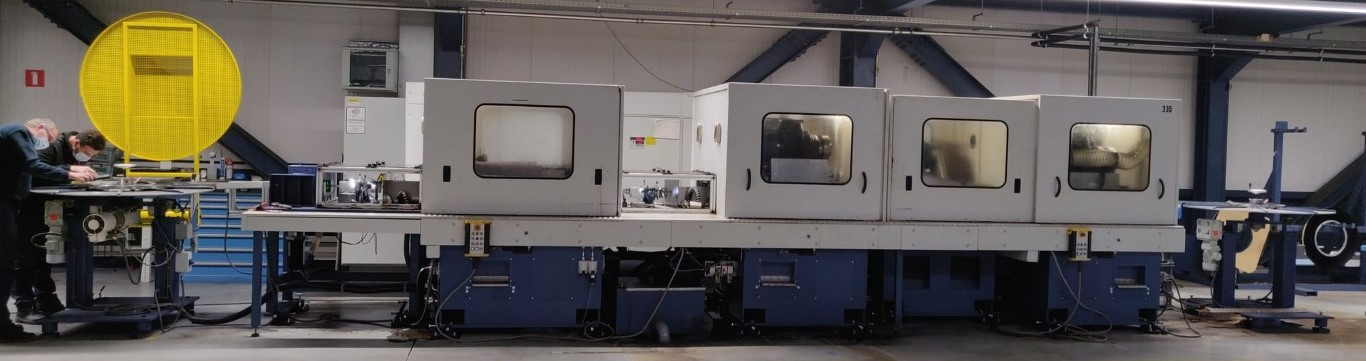
\includegraphics[width=0.95\linewidth]{stumabo/installation/line_photo.jpg}
        % \caption{Line overview: side view}
    \end{figure}
    \textbf{General goals}:
    \begin{itemize}
        \item Increase production quality
        \item Avoid unplanned standstill \& extend machines's life
        \item Identify the impact of the grindstones turning
        \item Find the root-cause of strong vibration
    \end{itemize}

    \vspace*{\fill}
\end{frame}

\begin{frame}
    \frametitle{Context}
    \begin{figure}[ht]
        \begin{subfigure}{\textwidth}
            \centering
            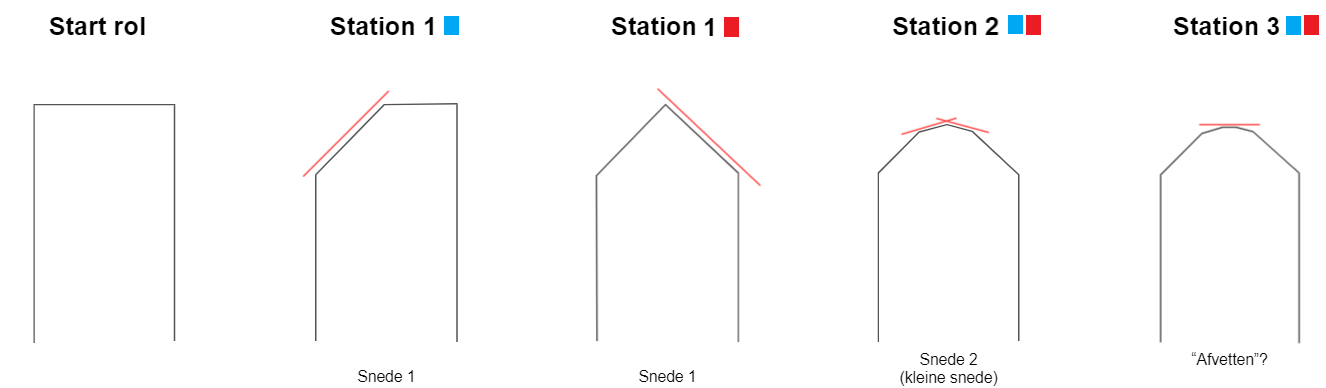
\includegraphics[width=0.65\textwidth]{stumabo/installation/blade_processing.png}
            % \caption{Blade evolution, a sketched overview of the cut by station}
        \end{subfigure}
        \begin{subfigure}{\textwidth}
            \centering
            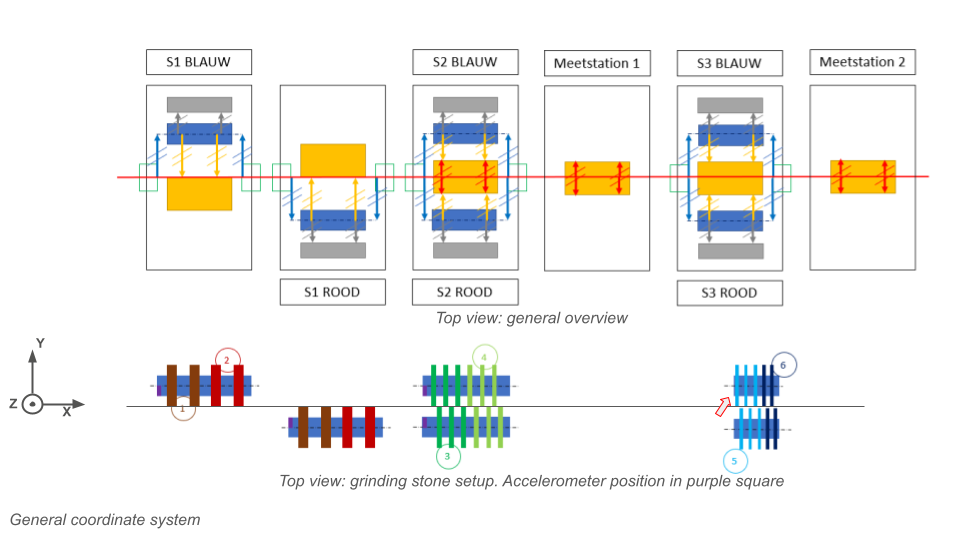
\includegraphics[width=0.67\textwidth]{stumabo/installation/general_cordinate_system.png}
            % \caption{Top view schematics}
        \end{subfigure}
        \caption{Blade evolution \& line top view; engineering schematics}
    \end{figure}
\end{frame}

% \subsection{4 Phases}
\begin{frame}
    \frametitle{4 Phases -- I}
    \vspace*{\fill}
    \begin{columns}[onlytextwidth, c]
        \begin{column}{.47\textwidth}
            \begin{exampleblock}{Hardware \& Data sources}
                \begin{itemize}
                    \item 3-dimension accelerometer
                    \item Mobile cabinet
                    \item Log file (operational data)
                \end{itemize}
            \end{exampleblock}
        \end{column}

        \begin{column}{.52\textwidth}
            \begin{figure}[ht]
                \begin{subfigure}{0.49\textwidth}
                    \centering
                    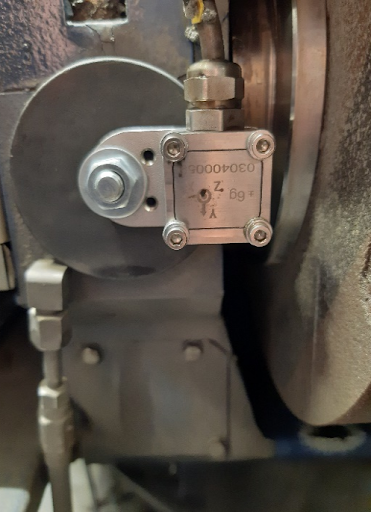
\includegraphics[height=\linewidth]{stumabo/installation/acc_station_1_blue.png}
                    \caption{Installation photo}
                \end{subfigure}
                \begin{subfigure}{0.49\textwidth}
                    \centering
                    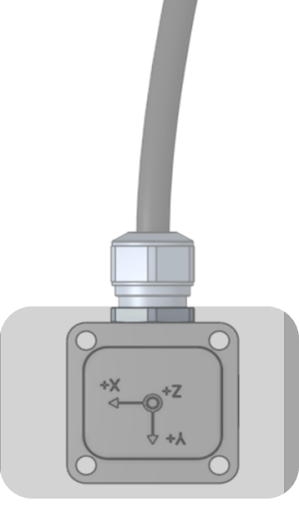
\includegraphics[height=\linewidth]{stumabo/installation/acc_render.png}
                    \caption{CAD render}
                \end{subfigure}
            \end{figure}
        \end{column}
    \end{columns}
    \vspace*{\fill}
\end{frame}

\begin{frame}
    \frametitle{4 Phases -- II}
    \vspace*{\fill}
    \begin{columns}[onlytextwidth, c]
        \begin{column}{.47\textwidth}
            \begin{exampleblock}{Installation}
                \begin{itemize}
                    \item \textcolor{red}{red} and \textcolor{blue}{blue} sides
                    \item Local $(x,y,z)$ for each sensor placement
                    \item Global $(X,Y,Z)$ for the entire production line
                    \item Sensor orientation and installation angle
                \end{itemize}
            \end{exampleblock}
        \end{column}
        \begin{column}{.52\textwidth}
            \begin{figure}
                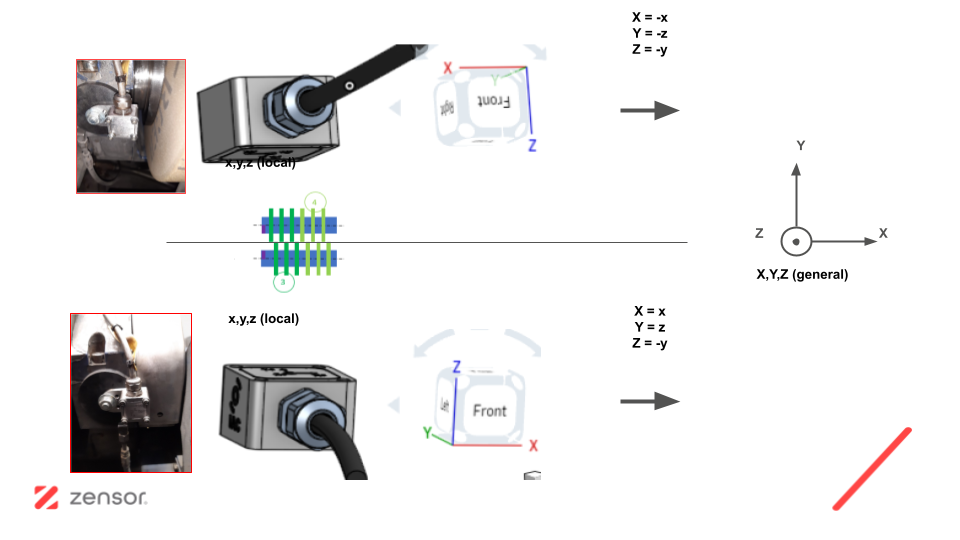
\includegraphics[width=\linewidth]{stumabo/installation/local_to_global.png}
                \caption{From local to general coordinate system}
            \end{figure}
        \end{column}
    \end{columns}
    \vspace*{\fill}
\end{frame}

\begin{frame}
    \frametitle{4 Phases -- III}
    \vspace*{\fill}
    \begin{columns}[onlytextwidth, c]
        \begin{column}{.47\textwidth}
            \begin{exampleblock}{Data Management}
                \begin{itemize}
                    \item Single data stream
                    \item  $ ACC_{x, y, z} \longrightarrow DB$
                    \item 60Hz to 1Hz /w Lambda
                \end{itemize}
            \end{exampleblock}
        \end{column}
        \begin{column}{.52\textwidth}
            \\
        \end{column}
    \end{columns}
    \begin{figure}[ht]
        \begin{subfigure}{0.495\textwidth}
            \centering
            \includegraphics[width=0.875\textwidth]{stumabo/analysis/60Hz-raw-vibration.pdf}
            \caption{60Hz raw vibration}
            \label{fig:stu_60Hz_raw}
        \end{subfigure}
        \begin{subfigure}{0.495\textwidth}
            \centering
            \includegraphics[width=0.875\textwidth]{stumabo/analysis/1Hz-raw-vibration.pdf}
            \caption{1Hz raw vibration}
            \label{fig:stu_1Hz_raw}
        \end{subfigure}
    \end{figure}
    \vspace*{\fill}
\end{frame}

\begin{frame}
    \frametitle{4 Phases -- IV}
    \vspace*{\fill}
    % Slide 1
    \begin{columns}[onlytextwidth, c]
        \begin{column}{.47\textwidth}
            \begin{exampleblock}{Analysis}
                \begin{enumerate}
                    \item \ac{EDA}
                    \item Isolate relevant blocks
                    \item Retrive ACC Data
                    \item Vector calculus: ${x, y, z} \rightarrow {X,Y,Z}$
                    \item \acl{RMS} (\acs{RMS})
                \end{enumerate}
            \end{exampleblock}
        \end{column}
        \begin{column}{.52\textwidth}
            \begin{figure}
                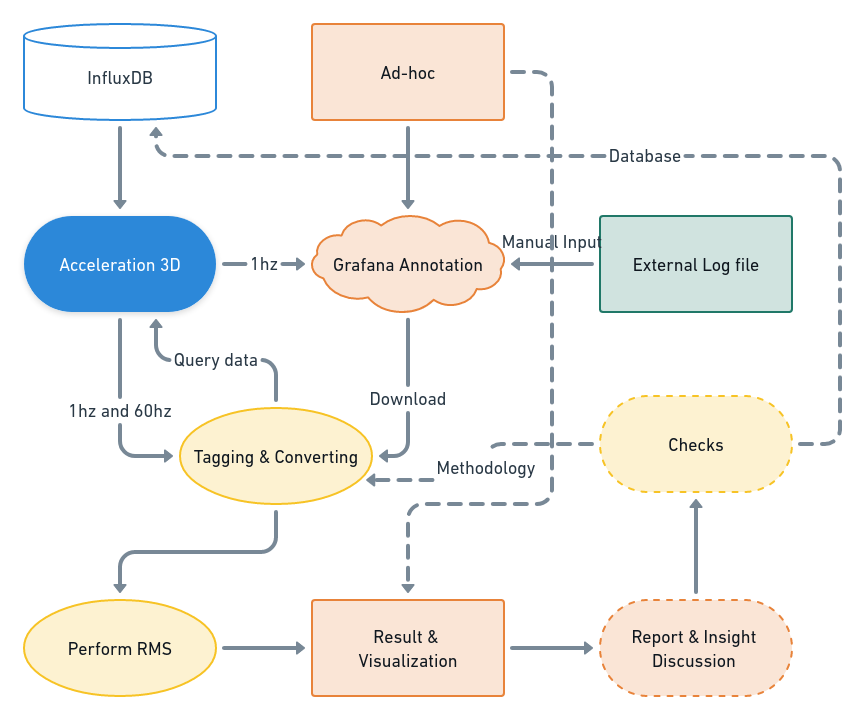
\includegraphics[width=\linewidth]{stumabo/analysis/analysis_flow.png}
                \caption{Steps involved during and after the analysis phase}
            \end{figure}
        \end{column}
    \end{columns}
    \vspace*{\fill}
\end{frame}

\begin{frame}
    \frametitle{Results}
    \vspace*{\fill}
    These plots were then discussed with a more experienced colleague, who had more domain knowledge.
    He also continued with the analysis.
    % decided not to discuss his insights, here
    % in this report, as they are not the result of my work but a more direct consequence.
    % Slide 2
    \begin{figure}[htp]
        \begin{subfigure}{.495\textwidth}
            \includegraphics[width=1.01\textwidth]{stumabo/analysis/1Hz-ad-hoc.pdf}
            \caption{1Hz RMS values}
            \label{fig:stu_1Hz_rms}
        \end{subfigure}
        \begin{subfigure}{.495\textwidth}
            \includegraphics[width=1.01\textwidth]{stumabo/analysis/60Hz-ad-hoc.pdf}
            \caption{60Hz RMS values}
            \label{fig:stu_60Hz_rms}
        \end{subfigure}
        % \begin{subfigure}{\textwidth}
        %     \includegraphics[width=\textwidth]{stumabo/analysis/1Hz-vs-60Hz.pdf}
        %     \caption{\texttt{1Hz} and \texttt{60Hz} RMS values}
        %     \label{fig:stu_1_vs_60}
        % \end{subfigure}
        \caption{RMS amplitude comparison \\between low and high frequency data}
        \label{fig:stu_3_rms}
    \end{figure}

    \vspace*{\fill}
\end{frame}

\begin{frame}
    \frametitle{Findings}
    \vspace*{\fill}

    The \textit{ad-hoc} analysis showed some insightful findings:
    \begin{enumerate}
        \item station one, \textcolor{blue}{blue} side, has higher vibration than expected
        \item station two is the main source of vibration as we hoped it would be
        \item the cooling fluid, while drying, cause higher vibrations.
    \end{enumerate}

    \begin{alertblock}{Counter-intuitive result}
        Vibration amplitudes ($RMS_{X}$), along the blade going through the grinding stone stations, seemed more
        prominent than in $Y$ direction, perpendicular to the blade direction.
    \end{alertblock}

    The stones turning would intuitively cause
    more vibrations perpendicular ($Y, Z$) to their rotating axe, not along $X$.\\
    After successfully double-checking the whole stack we can confirm that, indeed, $X$ and $Y$ are \structure{not} switched.
    \vspace*{\fill}
\end{frame}

% \section{Monitor electricity consumption}
\SectionPage

\begin{frame}
    \frametitle{Goals}
    \vspace*{\fill}
    Track the energy usage of a large campus, the \ac{BHC}, in Jette, using existing data collected over several years.
    We focus on the academic hospital, that has its own distribution network, in closed-ring shape for increased reliability.

    \textbf{General goals}:
    \begin{itemize}
        \item Having a global view on the data, centralized and well accessible for multiple user
        \item Minimizing the energy losses and overall consumption
        \item Identify where the exact sources of energy cost are
        \item Improve sustainability reducing energy need and peek request
    \end{itemize}

    \vspace*{\fill}
\end{frame}

\begin{frame}
    \frametitle{Context}
    \begin{figure}[ht]
        \fbox{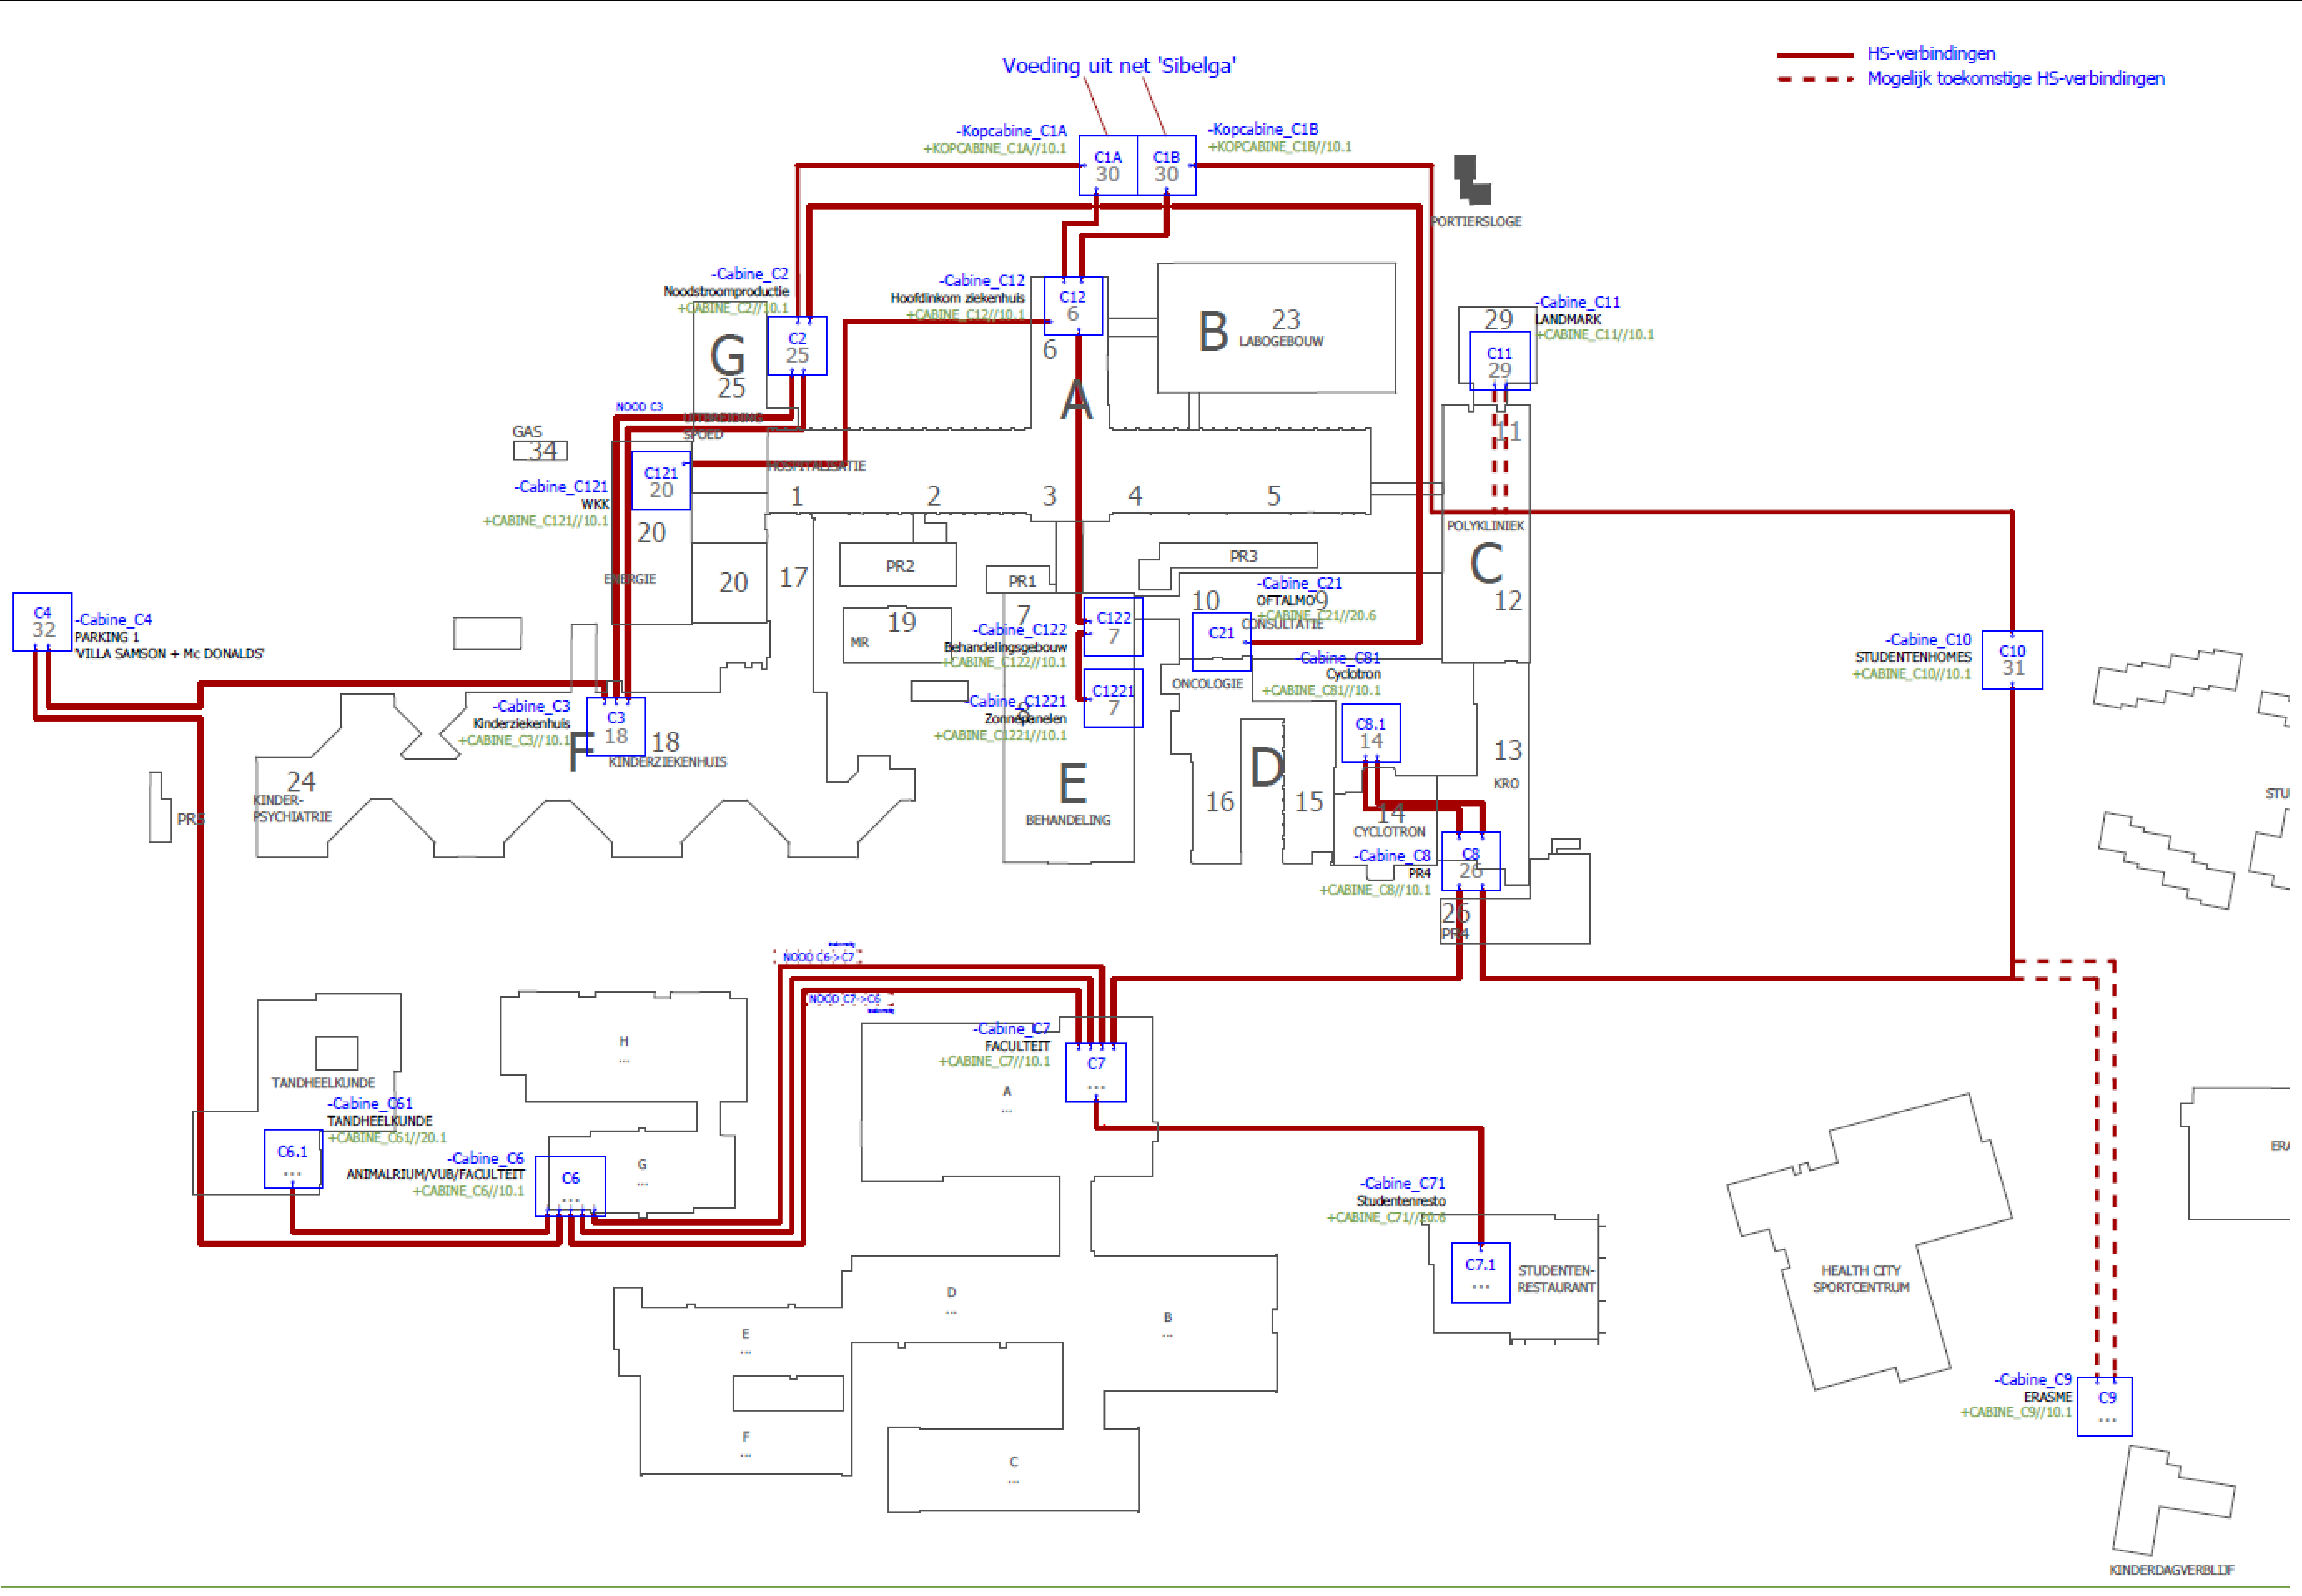
\includegraphics[width=0.78\textwidth]{vub/context/campus_site_layout.pdf}}
        \caption{\acs{UZB} electricity distribution network layout}
        \label{fig:bhc_site_layout}
    \end{figure}
\end{frame}

% \subsection{4 Phases}
\begin{frame}
    \frametitle{4 Phases -- I}
    \vspace*{\fill}
    \begin{columns}[onlytextwidth, c]
        \begin{column}{.47\textwidth}
            \begin{exampleblock}{Data sources}
                \begin{itemize}
                    \item Tries to reflect reality
                    \item Limited dataset
                    \item 15-minute ``electricity'' data
                    \item Also metedata source
                \end{itemize}
                Example:\\
                \texttt{root/NodeC3/Transformer\\
                    0302/ConsumerEnergy/\\
                    Bord\_Radiologie.csv}
            \end{exampleblock}
        \end{column}

        \begin{column}{.52\textwidth}
            \begin{figure}[ht]
                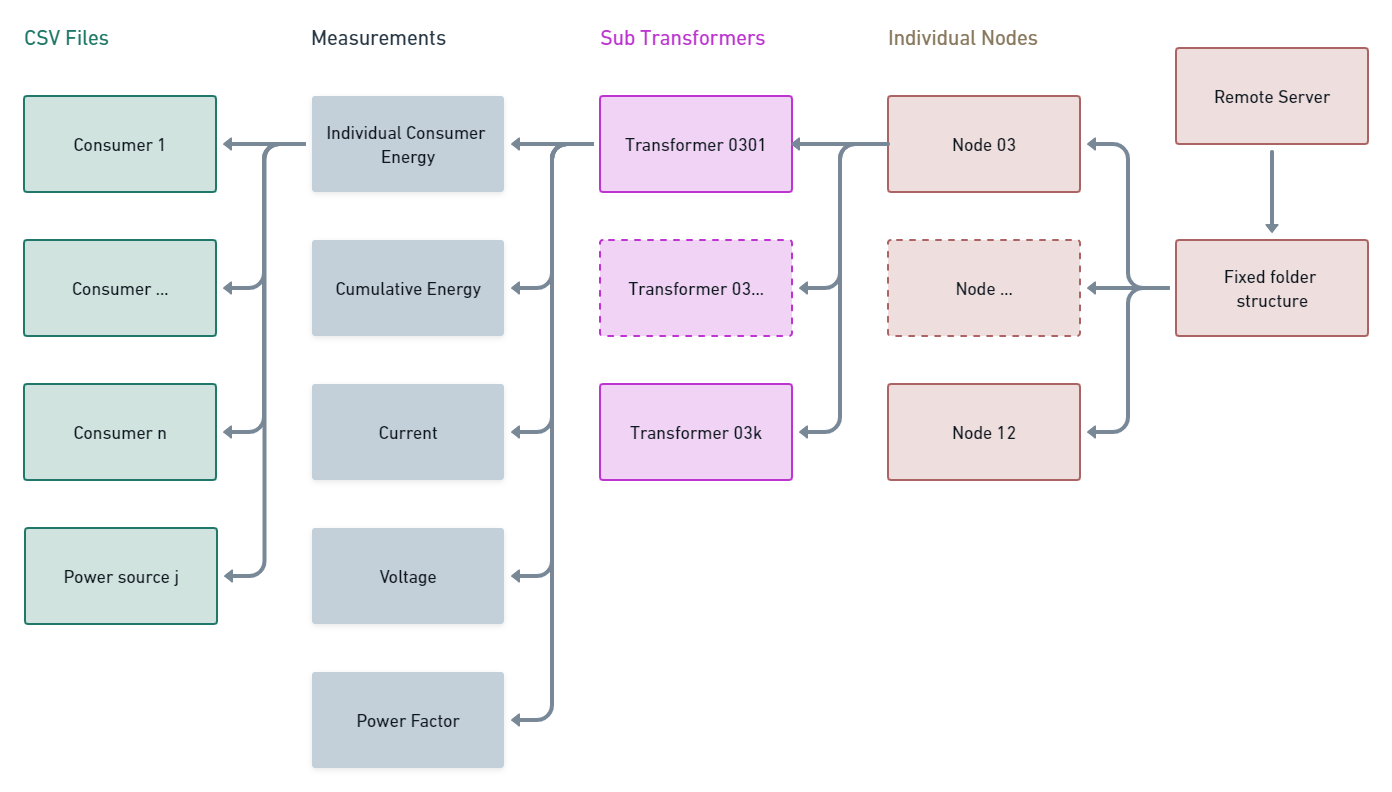
\includegraphics[width=\textwidth]{vub/flowcharts/folder_tree.png}
                \caption{\acs{VUB}'s folder tree structure}
            \end{figure}
        \end{column}
    \end{columns}
    \vspace*{\fill}
\end{frame}

\begin{frame}
    \frametitle{4 Phases -- II \& III}
    \vspace*{\fill}
    \begin{columns}[onlytextwidth, c]
        \begin{column}{.47\textwidth}
            \begin{exampleblock}{Commissioning}
                \begin{itemize}
                    \item \ac{SFTP}
                    \item automate remote access
                    \item automate ingestion
                \end{itemize}
            \end{exampleblock}
        \end{column}
        \begin{column}{.52\textwidth}
            \begin{exampleblock}{Data Management}
                \begin{itemize}
                    \item Multi processing script
                    \item Parsing, cleaning and tagging % w/ Pandas
                    \item Writing DB ``measurement''  %for each node
                \end{itemize}
            \end{exampleblock}
        \end{column}
    \end{columns}
    \begin{figure}[ht]
        \includegraphics[width=\textwidth]{vub/flowcharts/data-management.png}
        \caption{\acs{VUB}'s data ingestion flowchart}
    \end{figure}
    \vspace*{\fill}
\end{frame}

\begin{frame}
    \frametitle{4 Phases -- IV}
    \vspace*{\fill}
    \begin{columns}[onlytextwidth, c]
        \begin{column}{.47\textwidth}
            \begin{exampleblock}{Analysis}
                \begin{itemize}
                    \item Lorem
                    \item Ipsum
                    \item Sed 
                    \item Dolore
                \end{itemize}
            \end{exampleblock}
        \end{column}
        \begin{column}{.52\textwidth}
            \begin{figure}[ht]
                \begin{subfigure}{\textwidth}
                    \centering
                    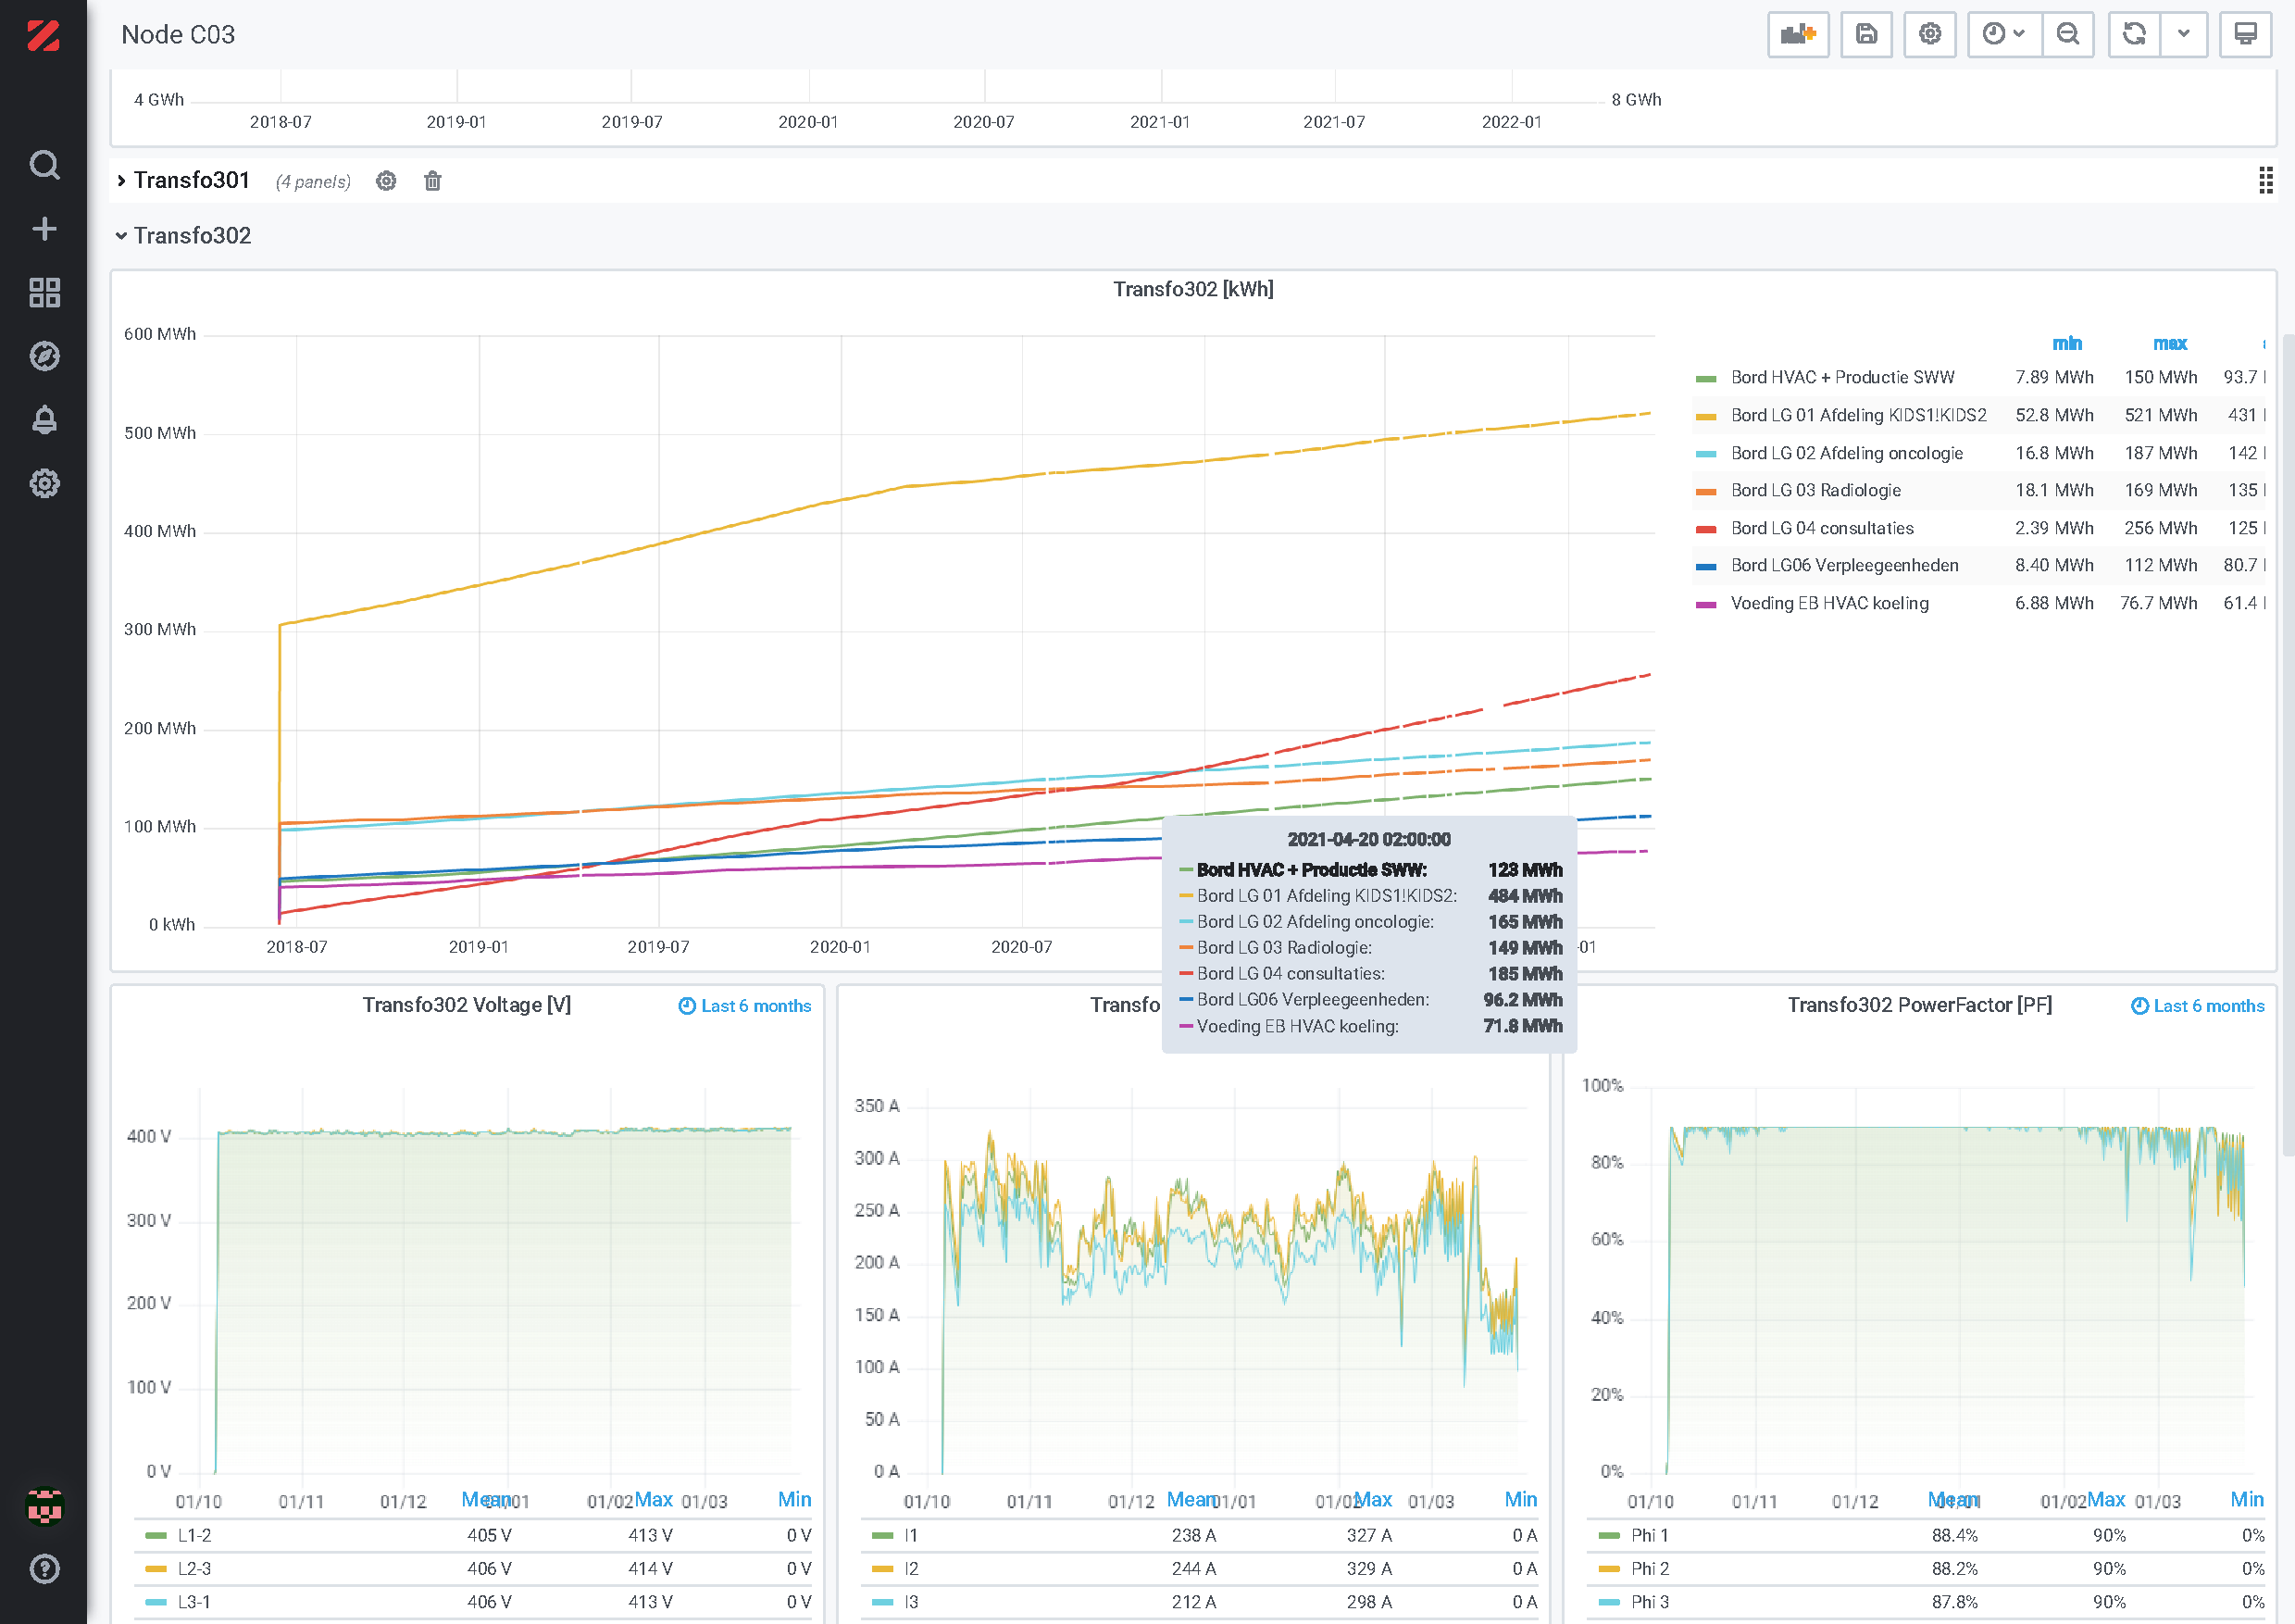
\includegraphics[clip, trim=0 0 0.1cm 3.5cm, width=0.8\textwidth]{vub/grafana/node_c03_transfo302_raw.pdf}
                    \caption{Transformer--302 raw data dashboard}
                \end{subfigure}
                \begin{subfigure}{\textwidth}
                    \centering
                    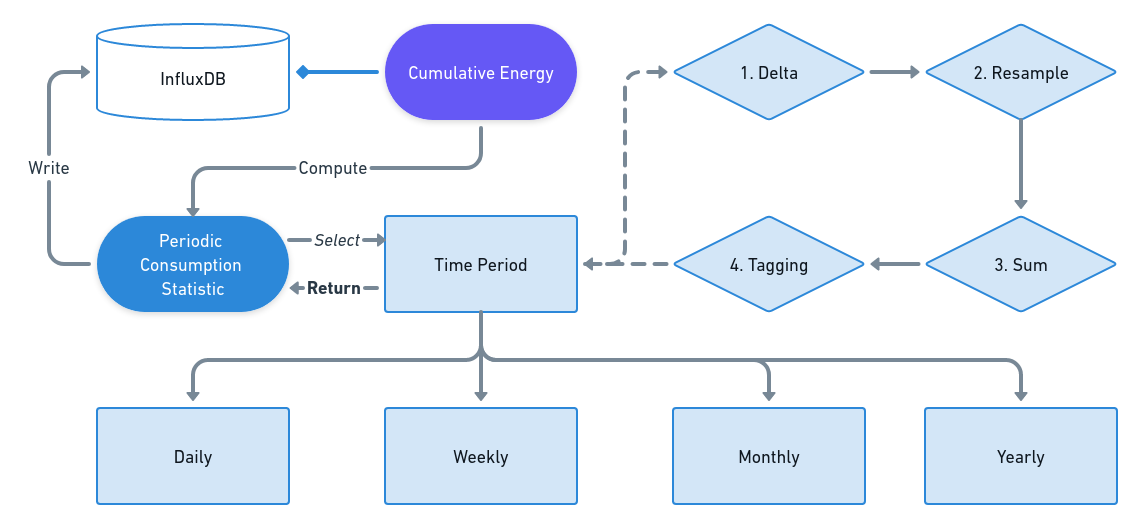
\includegraphics[width=0.8\textwidth]{vub/flowcharts/analystic_flowchart.png}
                    \caption{\acs{VUB}'s analytics chart}
                \end{subfigure}
            \end{figure}
        \end{column}
    \end{columns}
    \vspace*{\fill}
\end{frame}


% \begin{frame}
%     \frametitle{Results}
%     \vspace*{\fill}
%     These plots were then discussed with a more experienced colleague, who had more domain knowledge.
%     He also continued with the analysis.
%     % decided not to discuss his insights, here
%     % in this report, as they are not the result of my work but a more direct consequence.
%     % Slide 2
%     \begin{figure}[htp]
%         \begin{subfigure}{.495\textwidth}
%             \includegraphics[width=1.01\textwidth]{stumabo/analysis/1Hz-ad-hoc.pdf}
%             \caption{1Hz RMS values}
%             \label{fig:stu_1Hz_rms}
%         \end{subfigure}
%         \begin{subfigure}{.495\textwidth}
%             \includegraphics[width=1.01\textwidth]{stumabo/analysis/60Hz-ad-hoc.pdf}
%             \caption{60Hz RMS values}
%             \label{fig:stu_60Hz_rms}
%         \end{subfigure}
%         % \begin{subfigure}{\textwidth}
%         %     \includegraphics[width=\textwidth]{stumabo/analysis/1Hz-vs-60Hz.pdf}
%         %     \caption{\texttt{1Hz} and \texttt{60Hz} RMS values}
%         %     \label{fig:stu_1_vs_60}
%         % \end{subfigure}
%         \caption{RMS amplitude comparison between low and high frequency data}
%         \label{fig:stu_3_rms}
%     \end{figure}

%     \vspace*{\fill}
% \end{frame}


% \begin{frame}
%     \frametitle{Findings}
%     \vspace*{\fill}

%     The \textit{ad-hoc} analysis showed some insightful findings:
%     \begin{enumerate}
%         \item station one, \textcolor{blue}{blue} side, has higher vibration than expected
%         \item station two is the main source of vibration as we hoped it would be
%         \item the cooling fluid, while drying, cause higher vibrations.
%     \end{enumerate}

%     \begin{alertblock}{Counter-intuitive result}
%         Vibration amplitudes ($RMS_{X}$), along the blade going through the grinding stone stations, seemed more
%         prominent than in $Y$ direction, perpendicular to the blade direction.
%     \end{alertblock}

%     The stones turning would intuitively cause
%     more vibrations perpendicular ($Y, Z$) to their rotating axe, not along ($X$).\\
%     After successfully double-checking the whole stack we can confirm that, indeed, $X$ and $Y$ are \structure{not} switched.
%     \vspace*{\fill}
% \end{frame}
% \begin{frame}[]{Conclusion}{Important subtitle}
    
\end{frame}

\begin{frame}[plain]
    \vspace*{\fill}
    \begin{minipage}[c][0.63\paperheight]{\textwidth}
        \begin{figure}[ht]
            \begin{subfigure}{.495\textwidth}
                \centering
                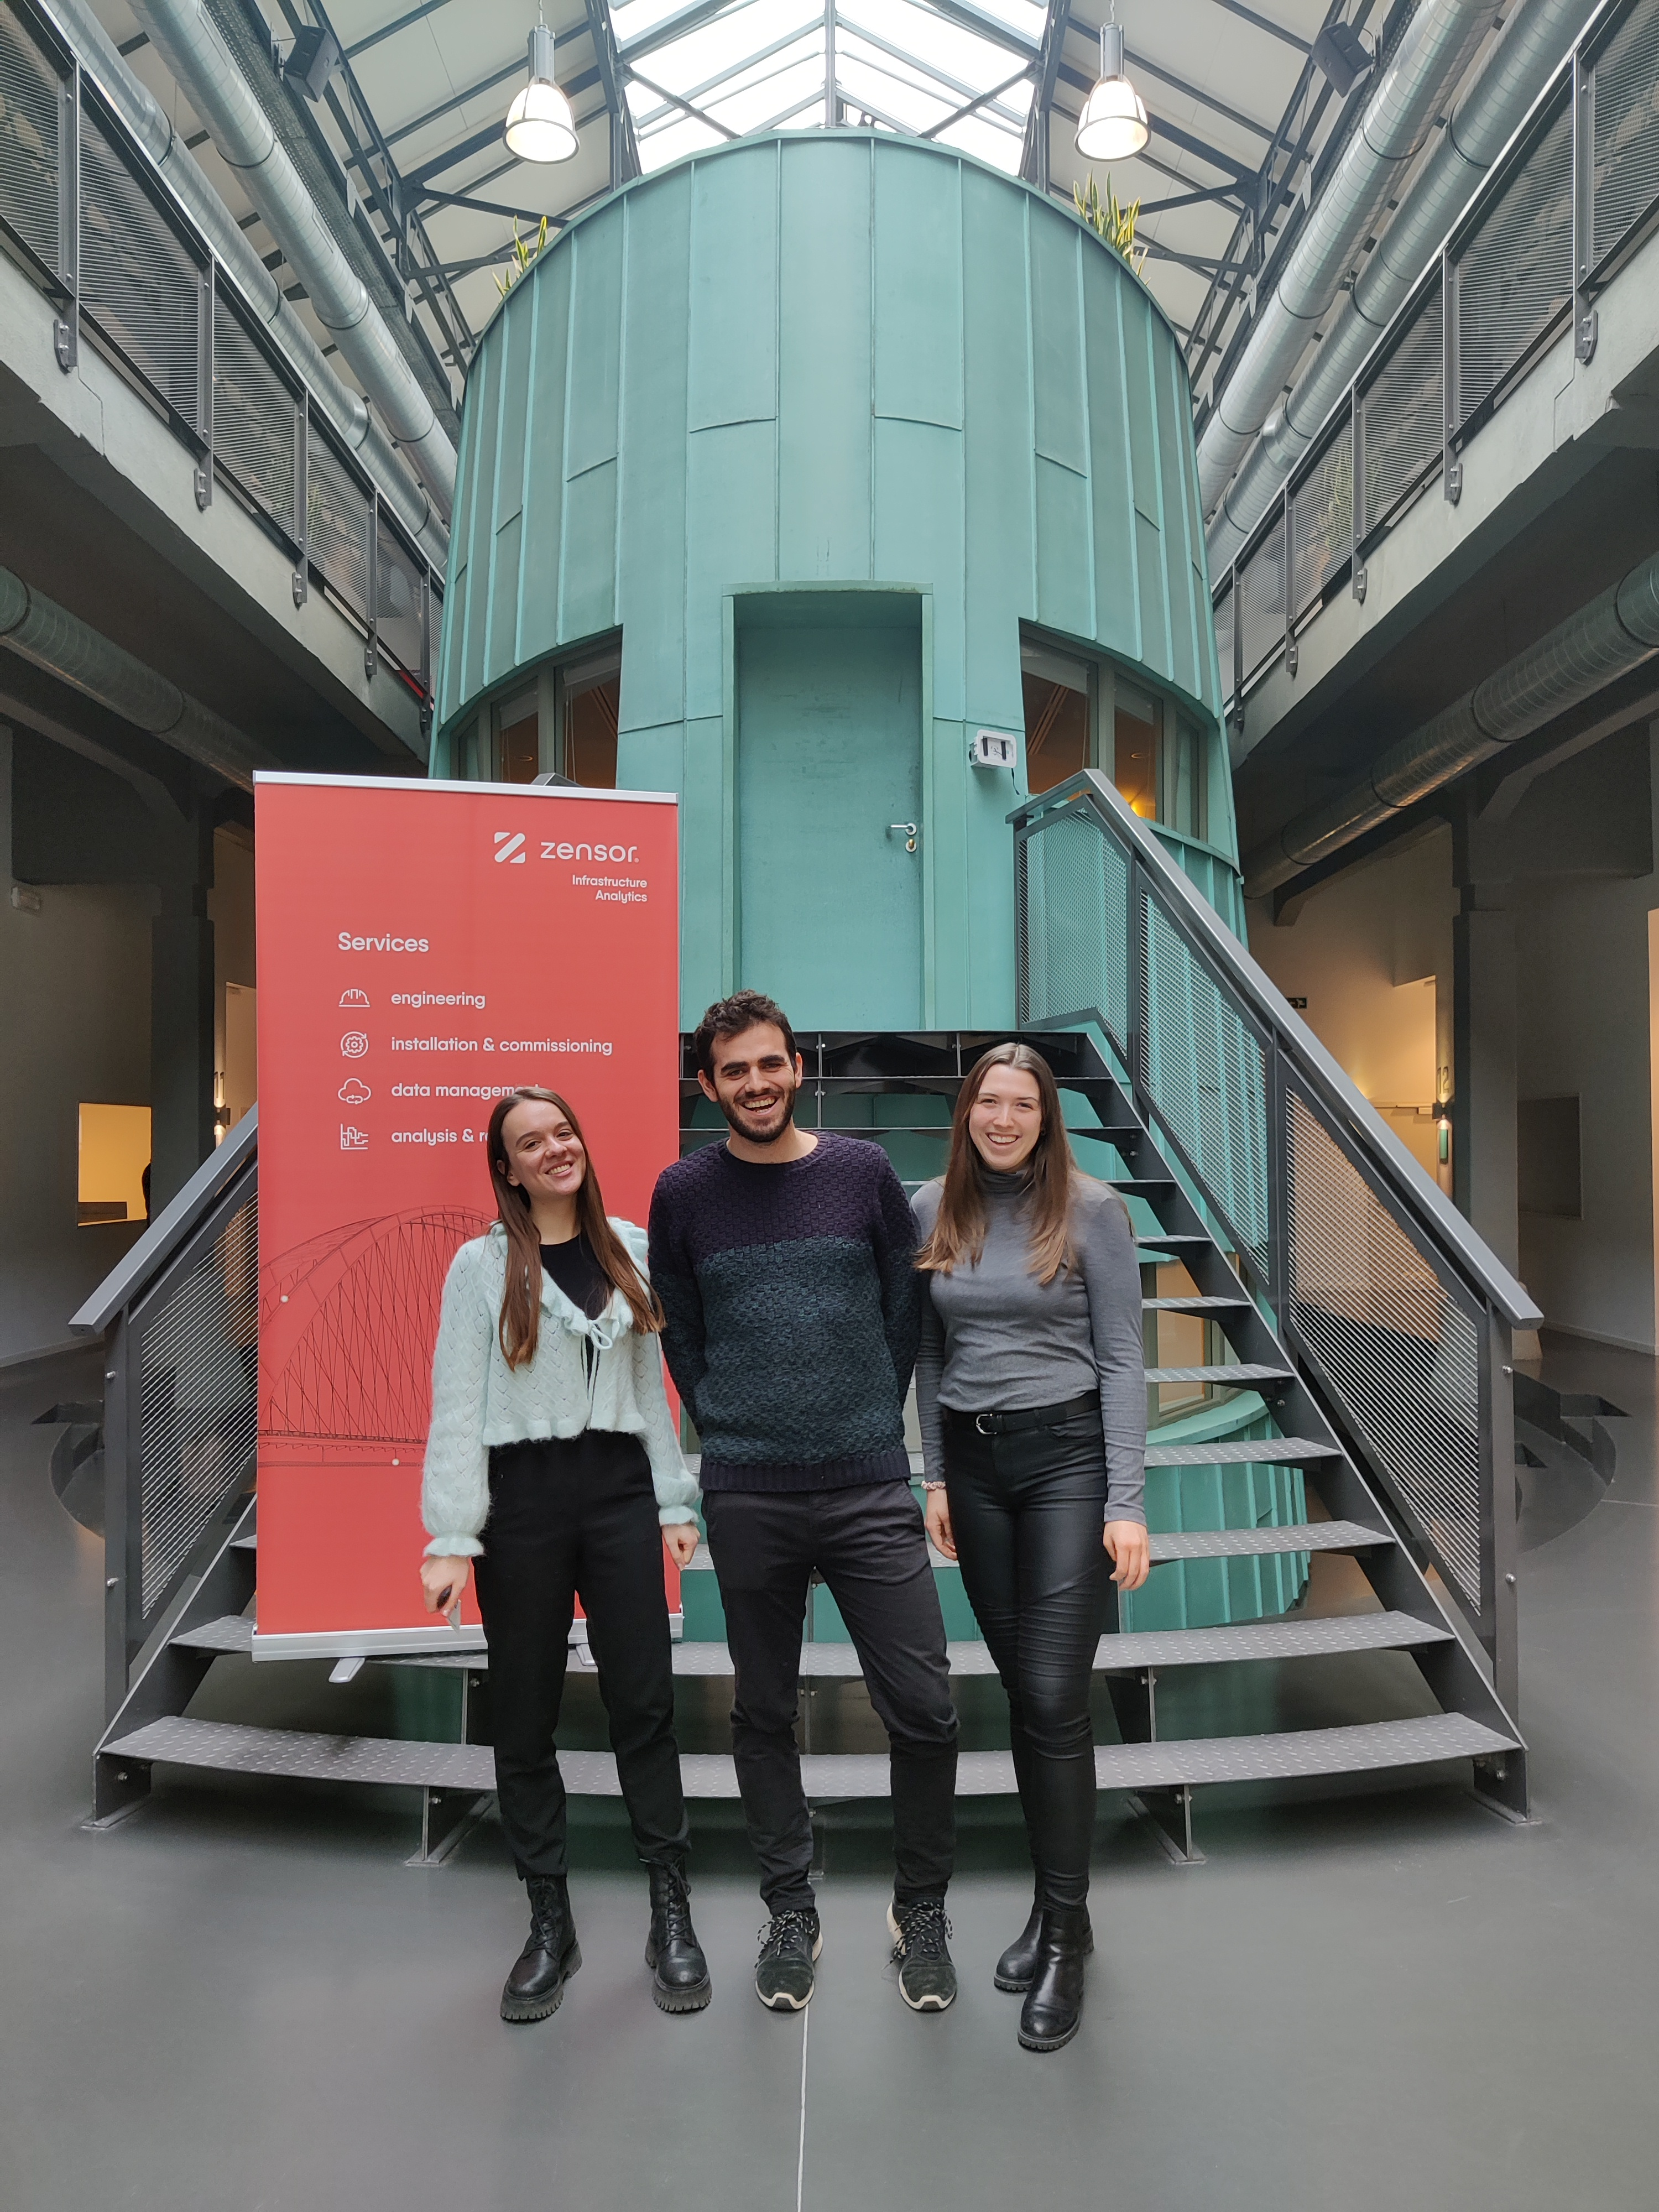
\includegraphics[width=0.7\textwidth]{icab.jpg}
            \end{subfigure}
            \begin{subfigure}{.495\textwidth}
                \centering
                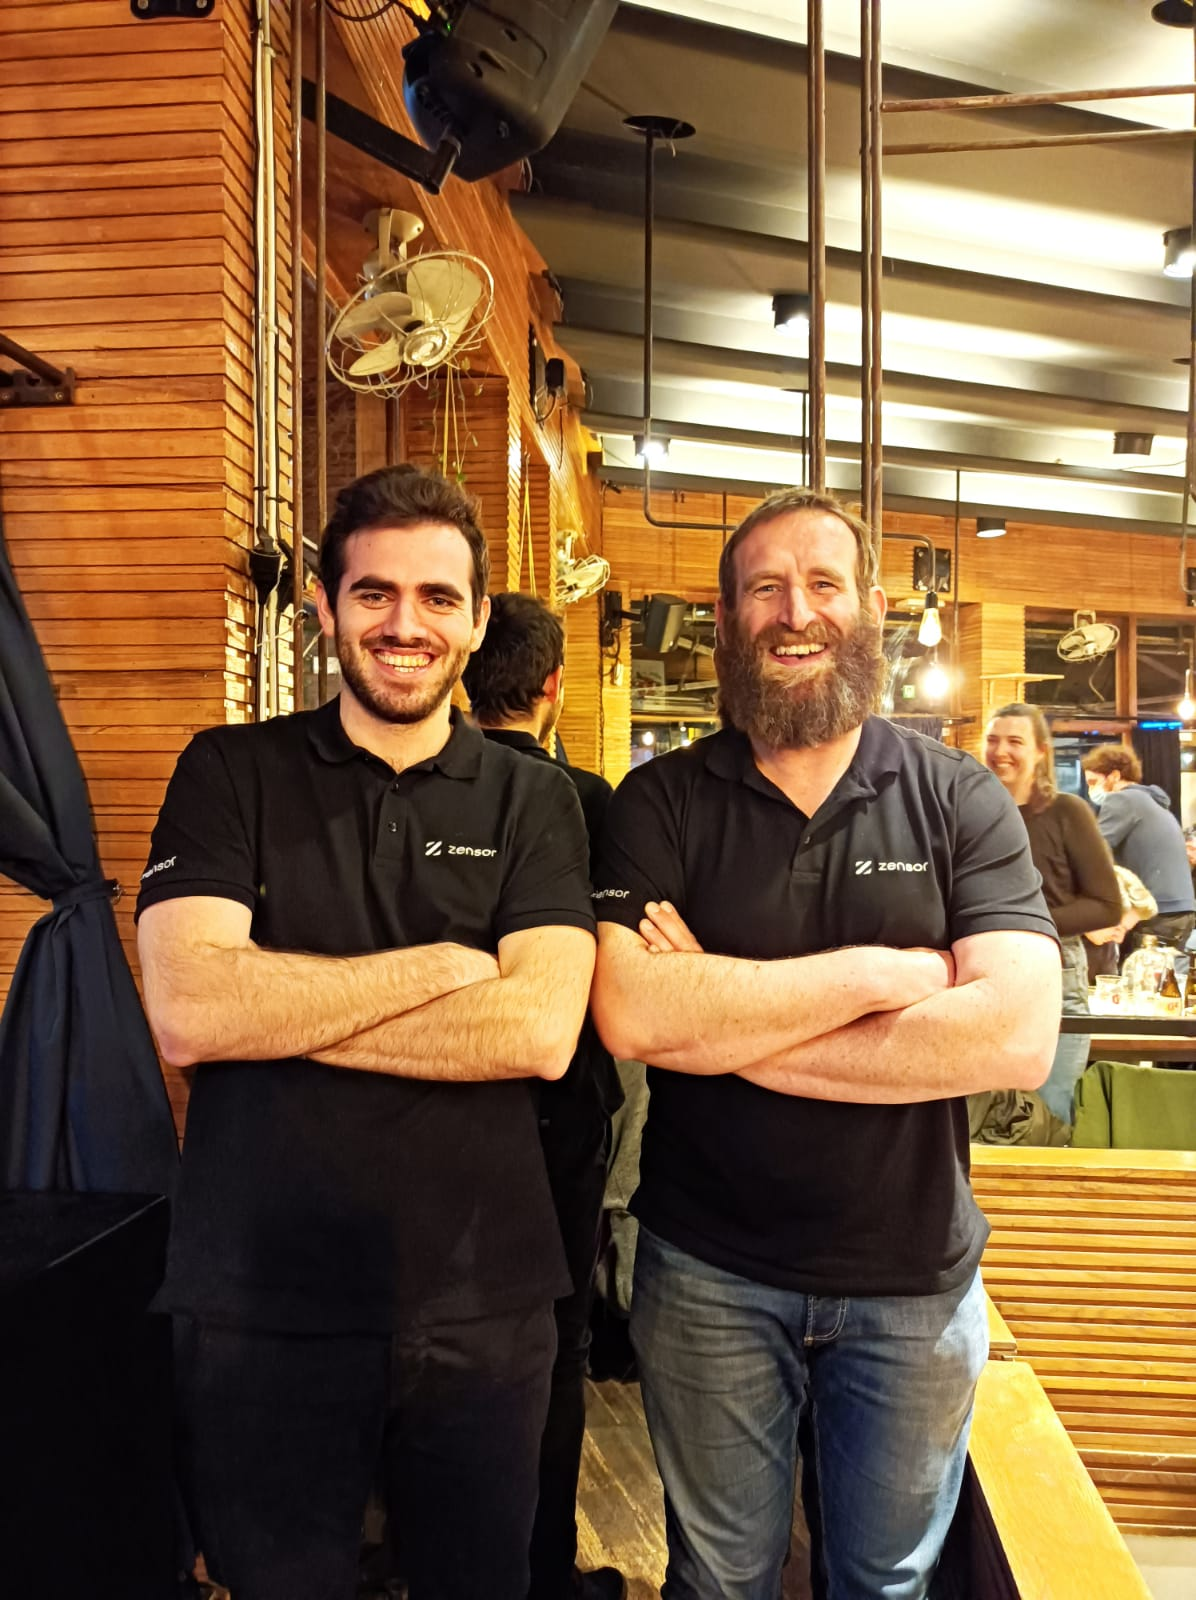
\includegraphics[width=0.7\textwidth]{dami_and_bart.jpg}
            \end{subfigure}
        \end{figure}
    \end{minipage}

    \begin{beamercolorbox}[wd        = \paperwidth,
            leftskip  = 1 em,
            rightskip = 1 em]
        {section in head/foot}

        \begin{minipage}[c][0.2\paperheight]{\textwidth}
            \centering \bfseries{\LARGE Grazie per l'attenzione}

        \end{minipage}
    \end{beamercolorbox}

    \begin{minipage}[c][0.1\paperheight]{\textwidth}
    \end{minipage}

    \begin{textblock}{1}(0.05, 0.89)
        
\includegraphics[width = 3cm]{zensor_logo.png}
    \end{textblock}

    \begin{textblock}{1}(0.69, 0.91)
        
\includegraphics[width = 3.3cm]{logo_erasmus.png}
    \end{textblock}

    \vspace*{\fill}
\end{frame}

% \section{Highlighting}
\SectionPage
\begin{frame}{Highlighting}
    Sometimes it is useful to \alert{highlight} certain words in the text.

    \begin{alertblock}{Important message}
        If a lot of text should be \alert{highlighted}, it is a good idea to put it in a box.
    \end{alertblock}

    It is easy to match the \structure{colour theme}.
\end{frame}

\begin{frame}{Lists}
    \begin{itemize}
        \item
        Bullet lists are marked with a red box.
    \end{itemize}

    \begin{enumerate}
        \item
        \label{enum:item}
        Numbered lists are marked with a white number inside a red box.
    \end{enumerate}

    \begin{description}
        \item[Description] highlights important words with red text.
    \end{description}

    Items in numbered lists like \enumref{enum:item} can be referenced with a red box.

    \begin{example}
        \begin{itemize}
            \item
            Lists change colour after the environment.
        \end{itemize}
    \end{example}
\end{frame}

\section{Effects}
\begin{frame}{Effects}
    \begin{columns}[onlytextwidth]
        \begin{column}{0.49\textwidth}
            \begin{enumerate}[<+-|alert@+>]
                \item
                Effects that control

                \item
                when text is displayed

                \item
                are specified with <> and a list of slides.
            \end{enumerate}

            \begin{theorem}<2>
                This theorem is only visible on slide number 2.
            \end{theorem}
        \end{column}
        \begin{column}{0.49\textwidth}
            Use \textbf<3->{textblock} for arbitrary placement of objects.

            \pause
            \medskip
            It creates a box
            with the specified width (here in a percentage of the slide's width)
            and upper left corner at the specified coordinate (x, y)
            (here x is a percentage of width and y a percentage of height).
        \end{column}
    \end{columns}
    
    \begin{textblock}{0.3}(0.45, 0.55)
        \includegraphics<1, 3>[width = \textwidth]{frames/logos/logo_unito_black.pdf}
    \end{textblock}
\end{frame}
\end{document}